\mySection{7.2 Comparing $\frac{\overline{Y}-\mu}{\sigma/\sqrt{n}}$ and $\frac{\overline{Y}-\mu}{S/\sqrt{n}}$}
%-------------- start slide -------------------------------%{{{ 7.17
\begin{frame}
	% {\S\: 7.2 Comparing $\frac{\overline{Y}-\mu}{\sigma/\sqrt{n}}$ and $\frac{\overline{Y}-\mu}{S/\sqrt{n}}$}

	\begin{center}
		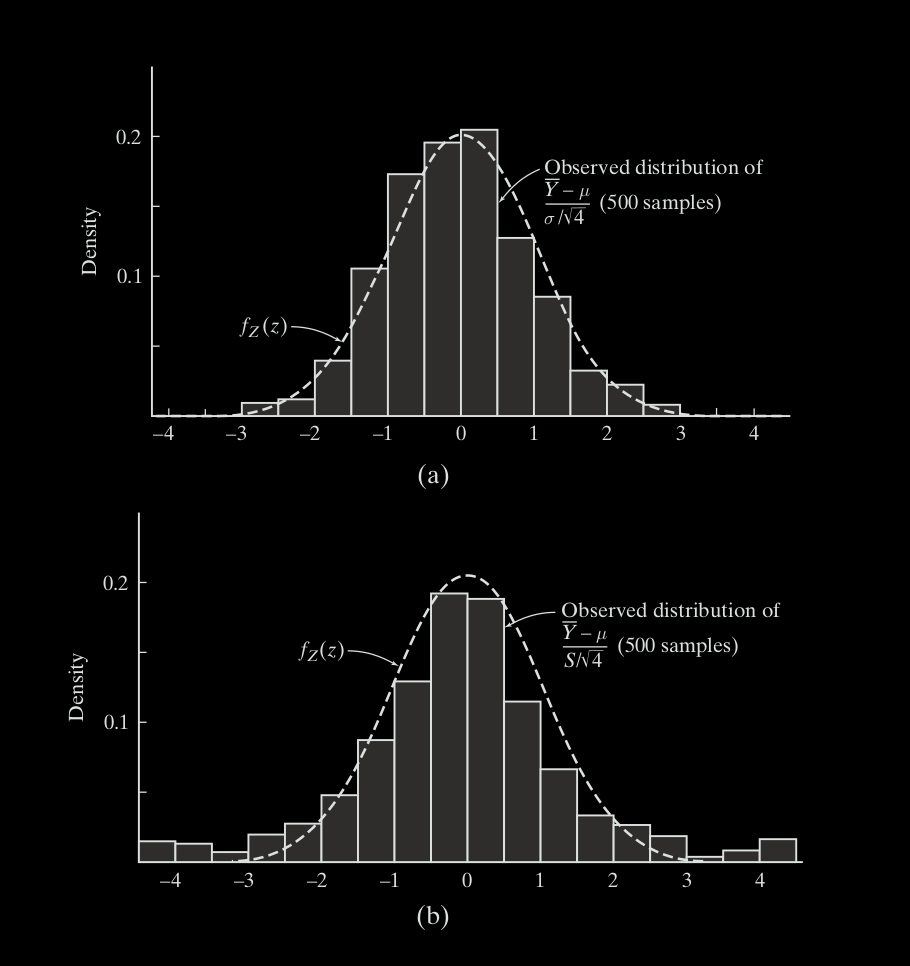
\includegraphics[scale=0.2]{Figure_7-2-1-neg.png}
	\end{center}
\end{frame}
%-------------- end slide -------------------------------%}}}
%-------------- start slide -------------------------------%{{{ 7.18
\begin{frame}
\centering
	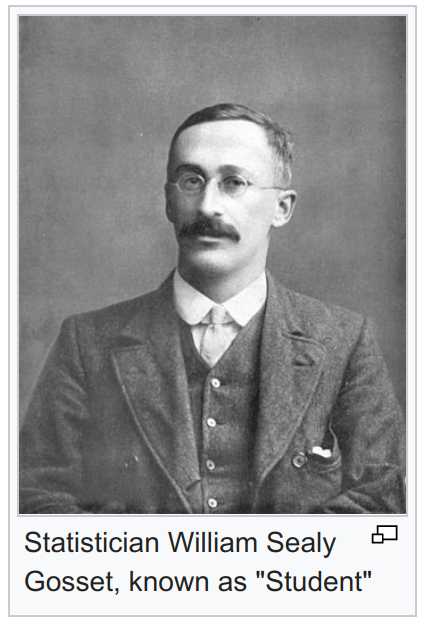
\includegraphics[scale=0.2]{Student.png}
	\hspace{3em}
	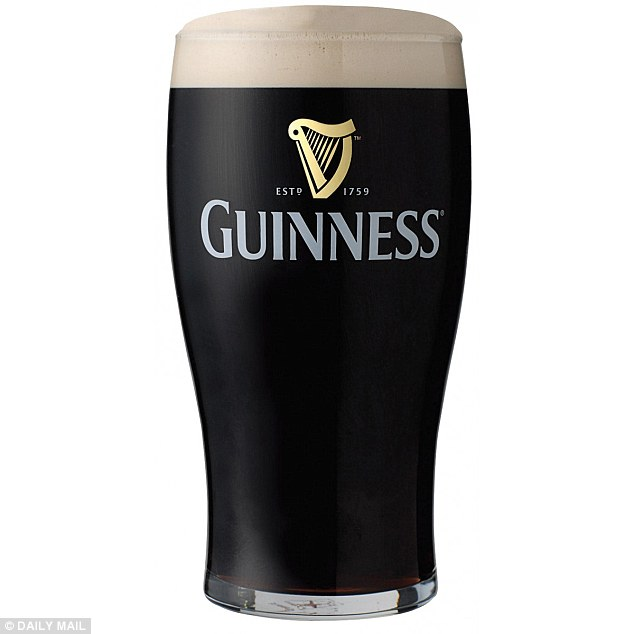
\includegraphics[scale=0.15]{Free-Pint-of-Guinness.png}
	\vfill
\footnotesize
	\begin{enumerate}
		\item[Ref.] Student's t distribution comes from William Sealy Gosset's 1908 paper in Biometrika under the pseudonym "Student".
		\item[] Gosset worked at the Guinness Brewery in Dublin, Ireland, and was interested in the problems of small samples -- for example, the chemical properties of barley where sample sizes might be as few as 3.
		\item[V1] One version of the origin of the pseudonym is that Gosset's employer preferred staff to use pen names when publishing scientific papers instead of their real name, so he used the name "Student" to hide his identity.
	\item[V2] Another version is that Guinness did not want their competitors to know that they were using the t-test to determine the quality of raw material
	\end{enumerate}
\end{frame}
%-------------- end slide -------------------------------%}}}
